\documentclass[11pt]{article}
\usepackage[margin=1in]{geometry}
\usepackage{amsmath,amssymb,amsthm,mathtools}
\usepackage{booktabs}
\usepackage{graphicx}
\usepackage{url}
\usepackage[colorlinks=true,linkcolor=blue,citecolor=blue,urlcolor=blue]{hyperref}
\hypersetup{pdftitle={The 262-operation 4x4x4:48 algorithm is also the more accurate one},pdfauthor={Greg Sidebottom}}
\newtheorem{theorem}{Theorem}[section]
\newtheorem{proposition}[theorem]{Proposition}
\newtheorem{lemma}[theorem]{Lemma}
\theoremstyle{remark}
\newtheorem{remark}[theorem]{Remark}
\newcommand{\Q}{\mathbb{Q}}
\newcommand{\Z}{\mathbb{Z}}
\newcommand{\R}{\mathbb{R}}
\newcommand{\Zh}{\Z[\tfrac12]}
\newcommand{\vect}{\operatorname{Vect}}
\newcommand{\Mat}{\operatorname{Mat}}
\newcommand{\nnz}[1]{\lVert #1\rVert_0}
\newcommand{\ginf}{\gamma_{\infty,2}}
\newcommand{\giinf}{\gamma_{\infty,\infty}}
\newcommand{\mm}[1]{\langle #1\rangle}
\usepackage{xspace}
\setlength{\emergencystretch}{1em}
\renewcommand{\topfraction}{0.85}
\renewcommand{\bottomfraction}{0.5}
\renewcommand{\textfraction}{0.15}
\renewcommand{\floatpagefraction}{0.75}
% schemes by their PLinOpt names
\newcommand{\acc}{\texttt{4x4x4\_\allowbreak 48\_\allowbreak accurate}\xspace}
\newcommand{\acct}{\texttt{4x4x4\_\allowbreak 48\_\allowbreak accurate\_\allowbreak 262}\xspace}
\newcommand{\rat}{\texttt{4x4x4\_\allowbreak 48\_\allowbreak rational}\xspace}
\newcommand{\pto}{\texttt{4x4x4\_\allowbreak 48\_\allowbreak 201}\xspace}
\title{The 262-operation $\mm{4\times4\times4:48}$ algorithm is also the\\
more accurate one: error-bound exponent $9/4$ and about a quarter
less error}
\author{Greg Sidebottom}
\date{Draft --- October 27, 2026}

\begin{document}
\maketitle

\begin{abstract}
Dumas, Pernet and Sedoglavic's accurate rational $\mm{4\times4\times4:48}$
algorithm (Table~1 of their 2026 paper; \acc in PLinOpt) has
$(\infty,2)$-growth factor
$\ginf=18\sqrt2\approx25.46$, an error-bound exponent $\log_4\ginf\approx2.335$.
Their later $262$-operation variant \acct, in the same orbit, was published for
its lower operation count.  We show that it is also the more accurate
algorithm.  Its growth factors are smaller in all four norms they
consider: $\ginf=16\sqrt2$, an exponent of exactly $9/4$;
$\giinf=132$ against $148$; $\gamma_{2,\infty}=16\sqrt{963}$ against
$8\sqrt{4142}$; and $\gamma_{2,2}=64\sqrt2$ against $8\sqrt{130}$.  Its
$\gamma_2=64(1+\sqrt2)$ is the same, and the combinatorial factor $Q_0$
of their error bounds is $34$ against $46$.  Measured against exact references on random
matrices, in single and double precision at one to three recursion
levels, its error is $0.75$--$0.77$ of \acc's on average ($0.62$--$0.90$ for single instances), at the same speed in a
fused-pass implementation over Apple's Accelerate.  In recursion down to scalars its advantage grows,
to $0.72$ at five levels.  We also minimize $\ginf$ over the whole
de~Groote orbit of the scheme and its three role assignments, with an
exact-gradient search.  The orbit's minimum is $\ginf=21.41$, exponent
$2.210$, reached in the two other role assignments at points whose
coefficients lie in $\Q(\sqrt2)$; in the published role the minimum is
$16\sqrt2$, at points equivalent to \acct, which we found before we
knew of it.  Among the orbit's $648$ dyadic orthogonal points, enumerated
exhaustively, the points minimizing both $\ginf$ and $\giinf$ are all
equivalent to \acct.  The $21.41$ point cannot be made dyadic, and in
floating point, where its constants round, its measured error is no
lower than \acc's.  Dyadic probe points show that neither $\ginf$ nor
$\giinf$ alone predicts the measured error, while $Q_0$ and exact dyadic
coefficients matter.  A first-order rounding model of the programs,
taken as a search objective, gives programs with $11\%$ less modelled
rounding error that measure as a tie, because the leaf products' error,
amplified by the scheme, dominates; that amplification, $2\sqrt2$ per
level, is the minimum over the orbit, over the other known rank-$48$
classes and over the variety of decompositions around them.  Adding in
double precision inside the single-precision passes, at no cost below
$n=16384$, cuts the error at five recursion levels by a third.  The
other known
rational classes, Li, Wang and Hu's curve and Agarwal's scheme, have
larger $\ginf$ minima.
\end{abstract}

\section{Introduction}\label{sec:intro}

Two $4\times4$ matrices can be multiplied with $48$ multiplications over
any ring containing $1/2$.  AlphaEvolve found a rank-$48$ scheme with
complex coefficients~\cite{Novikov25}, and Dumas, Pernet and Sedoglavic
(DPS) turned it into one with rational coefficients~\cite{DPS25}.
Applied recursively, such a scheme multiplies $n\times n$ matrices with
$O(n^{\log_4 48})=O(n^{2.7925})$ operations.  Fast schemes trade
accuracy for speed, and their error bounds are governed by a
\emph{growth factor} computed from the scheme's coefficient
matrices~\cite{Brent70,BL80,DDHK07,Higham02}.  DPS generalized it to a
$(p,q)$-growth factor $\gamma_{p,q}$ for any output and input
norms~\cite{DPS24,DPS26b}, and they argue that the
$(\infty,2)$-factor $\ginf$ best reflects the accuracy observed in
practice.

In~\cite{DPS26a} DPS proposed an accurate variant of their rational
scheme, given as Table~1 of that paper and in PLinOpt as
\acc~\cite{PLinOpt}.  They found it in the de
Groote isotropy orbit~\cite{deGroote78} of their first scheme: a point
minimizing the smooth bound $\gamma_2\ge\gamma_{2,2}$ along the orbit,
then moved by orthogonal isotropies, which keep $\gamma_2$, to get
sparse straight-line programs.  Its growth factor is $\ginf\approx25.456$,
error-bound exponent $\log_4\ginf\approx2.335$, the smallest among the
algorithms they compare, and its programs take $284$ operations.  The
paper's versions run from 19~March 2026 (v1) to 29~July 2026 (v3, the
current one), and \acc entered PLinOpt on 23~June 2026.

A cheaper accurate variant, with $262$ operations, came next.  Its
earliest trace is the second version of~\cite{DPSST26}, dated
2~October 2026, whose introduction states, without a reference or
coefficients, that the best currently known accurate variant has
leading term $9+3/16$, or $5+3/4$ in an alternative basis.  The leading
term is $1+q/32$ for $q$ additions, subtractions and scalings, so
$9+3/16$ means $q=262$.  The first version, of 10~September 2026,
mentions only \acc (leading term $9.875$).  The scheme itself was first
published in PLinOpt on 13~October 2026 as \acct (commit
\texttt{b441528}, by J.-G.~Dumas), described as ``accurate with 262
operations, or (5+3/4) ALT/CoB''.  Neither source says how it was
found or reports its growth factors, and \acc remains the accurate
variant on record.  After this paper's first draft, A.~Sedoglavic
informed us that the point with $\ginf=16\sqrt2$ was found by Touko
Ursin in mid-September 2026, by a construction with Hadamard matrices
(a reduced form of the parametrization of Section~\ref{sec:search})
rather than by search, and has not been published
yet~\cite{Sedoglavic26}.  In a second message he describes the
construction~\cite{Sedoglavic26b}: \acc is the orbit's $\gamma_2$
minimum, unique modulo orthogonal isotropies by their convexity result
and found by numerical optimization (pymanopt) over the quotient of
$GL_4$ by the orthogonal group~\cite[Lemma~27]{DPS26b}; Ursin then
explored the action of Hadamard matrices, orthogonal isotropies that
leave $\gamma_2$ unchanged, to lower $\ginf$, which gave \acct.

We call schemes by their PLinOpt names: \acc for Table~1
of~\cite{DPS26a}, \acct for the variant with $262$ operations, \rat for the
first rational scheme~\cite{DPS25}, \pto for our $201$-operation
point~\cite{S26}, and \texttt{2x2x2\_\allowbreak 7\_\allowbreak Winograd},
\texttt{2x2x2\_\allowbreak 7\_\allowbreak Strassen} and \texttt{2x2x2\_\allowbreak 7\_\allowbreak DPS-accurate} for the
$\mm{2\times2\times2:7}$ algorithms.  Tables drop the common prefixes.
Points of our search that are not in PLinOpt have descriptive names.

We show that \acct, the cheaper variant, is also the more accurate one:
\begin{itemize}
\item Its growth factors are smaller than \acc's in all four norms
  of~\cite[Table~2]{DPS26a}, with the same $\gamma_2$: $\ginf=16\sqrt2$,
  an error-bound exponent of exactly $9/4$, against $25.456$;
  $\giinf=132$ against $148$; $\gamma_{2,2}=64\sqrt2$ against $91.21$;
  and $\gamma_{2,\infty}\approx496.5$ against $514.9$.  The combinatorial
  factor $Q_0$ of DPS's error bounds is $34$ against $46$ (Section~\ref{sec:scheme}).
\item Measured on random matrices against exact references, in single
  and double precision, its error is $0.75$--$0.77$ of \acc's on average at one to
  three recursion levels, and never above $0.90$.  In recursion down to
  scalars the advantage grows, to $0.72$ at five levels.  It runs at the same speed in a fused-pass
  implementation over Apple's Accelerate (Sections~\ref{sec:acc}
  and~\ref{sec:speed}).
\end{itemize}

Before we knew of \acct, which was first published in PLinOpt (commit
\texttt{b441528}~\cite{PLinOpt}) and first found by Ursin
(Section~\ref{sec:intro}), our search found a scheme equivalent
to it, that is, \acct written in another way (Section~\ref{sec:inv}).
The search minimizes $\ginf$ over the orbit and the scheme's role
assignments (Section~\ref{sec:search}).  That search, and the value of
the orbit's $\ginf$ minimum it gives, are the paper's other
contribution.  In the published role the lowest point the search finds
is equivalent to \acct, and it is exact as found: its $U$ and $W$ have entries
$0,\pm1/\sqrt2$, which rescaling turns into dyadic coefficients, so no
snapping to a dyadic grid is involved.  Among the orbit's dyadic orthogonal points, which we
enumerate exhaustively, the points minimizing $\giinf$ also minimize
$\ginf$, and all of them are equivalent to \acct.  The orbit's global $\ginf$ minimum, $21.407$, is reached only
in the other two role assignments and only
at points with coefficients in $\Q(\sqrt2)$, and its measured error is
no lower than \acc's.  The other known rational classes, members of Li, Wang
and Hu's curve~\cite{LWH26} and Agarwal's scheme~\cite{Agarwal26}, have
larger $\ginf$ minima.  So $\ginf$ alone is not a sufficient objective
for an accuracy search.  The combinatorial factor $Q_0$ and exact
dyadic coefficients matter as much.  \acct has dyadic coefficients and
the smallest $Q_0$ and $\giinf$ of the $\mm{4\times4\times4:48}$ schemes
we measured.

\section{Background}\label{sec:background}

\subsection{Schemes, growth factors and $Q_0$}

For an $m\times k$ matrix $A$, $\vect(A)$ is its row-major
vectorization.  A bilinear algorithm with $r$ multiplications for
$\mm{m\times k\times n}$ is a triple of matrices $L\in\Q^{r\times mk}$,
$R\in\Q^{r\times kn}$, $P\in\Q^{mn\times r}$ with
\begin{equation}\label{eq:bilinear}
\vect(AB)=P\bigl((L\vect A)\odot(R\vect B)\bigr)
\end{equation}
for all $A$ and $B$, where $\odot$ is the entrywise product.  Here
$m=k=n=4$ and $r=48$.  With $L_i$ the rows of $L$, $R_i$ the rows of
$R$, $p_{j,i}$ the entries of $P$ and $q^\star$ the dual exponent of
$q$, DPS's $(p,q)$-growth factor~\cite[Def.~11]{DPS26b} is
\begin{equation}\label{eq:gamma}
\gamma_{p,q}=\Bigl\lVert\Bigl(\sum_{i=1}^{r}\lVert L_i\rVert_{q^\star}
\lVert R_i\rVert_{q^\star}\,\lvert p_{j,i}\rvert\Bigr)_{j}\Bigr\rVert_p ,
\end{equation}
and the forward error of $\ell$ recursive levels is at most
$f_{p,q}\lVert A\rVert_q\lVert B\rVert_q\,\varepsilon+O(\varepsilon^2)$
with $f_{p,q}=O(\gamma_{p,q}^{\ell})=O(n^{\log_4\gamma_{p,q}})$~\cite[Th.~18]{DPS26b}.  The
classical algorithm has $\giinf=\ginf=4$ and
$\gamma_{2,\infty}=\gamma_{2,2}=16$, exponents $1$ and $2$.  DPS also use the
smooth bound $\gamma_2=\sum_i\lVert L_i\rVert_2\lVert R_i\rVert_2
\lVert P_{*,i}\rVert_2\ge\gamma_{2,2}$~\cite[eq.~(5)]{DPS26a}.
The constant of their bounds also carries a combinatorial factor,
after Ballard et al.~\cite[Def.~1]{BBDLS16} (\cite[Th.~12]{DPS24},
\cite[Th.~18]{DPS26b}):
\begin{equation}\label{eq:q0}
Q_0=\max_j\Bigl(\nnz{P_j}+\max_{i:\,p_{j,i}\ne0}\bigl(\nnz{L_i}+\nnz{R_i}\bigr)\Bigr),
\end{equation}
where $\nnz{\cdot}$ counts nonzeros.  For the worst output it counts
the nonzeros of the worst product's two linear forms and the products
summed into the output, a crude count of the roundings a level exposes
the output to when the scheme is computed as direct sums: $Q_0-3$
additions and one multiplication.  The bounds multiply it by
$\gamma/(\gamma-k)$, which adds up the levels.  PLinOpt's
\texttt{growthfactor} tool~\cite{PLinOpt} (commit \texttt{cf85c3f}, May
2026, unchanged at \texttt{7c20065}) prints under the name $Q_0$ a
different quantity, the term count
\begin{equation}\label{eq:t0}
T_0=\max_j\Bigl(\max_{i:\,p_{j,i}\ne0}\nnz{L_i}\,\nnz{R_i}+\nnz{P_j}\Bigr),
\end{equation}
the terms $a_kb_l$ of the worst product feeding the output plus the
products summed into it: for Winograd's $\mm{2\times2\times2:7}$
algorithm it prints $13$ where \cite{DPS24} tabulates $Q_0=10$.
Table~\ref{tab:gamma} reports $Q_0$ as in~(\ref{eq:q0});
Section~\ref{sec:disc} uses $T_0$ once.

\subsection{Isotropies and symmetries}

For $(U,V,W)\in GL_4^3$, applying an algorithm to $U^{-1}AV$ and
$V^{-1}BW$ returns $U^{-1}ABW$, so
\begin{equation}\label{eq:act}
(L,R,P)\;\mapsto\;\bigl(L\,(U^{-1}\otimes V^{\mathsf T}),\;
R\,(V^{-1}\otimes W^{\mathsf T}),\;(U\otimes W^{-\mathsf T})\,P\bigr)
\end{equation}
is again an algorithm, since $\vect(XAY)=(X\otimes Y^{\mathsf T})\vect A$
for row-major vectorization.  These are de~Groote's
isotropies~\cite{deGroote78}; PLinOpt's orbit tool uses the same group.
With $A_i=\Mat(L_i)$, $B_i=\Mat(R_i)$ and $Z_i$ the $4\times4$ matrix of
column $i$ of $P$, (\ref{eq:act}) reads
\begin{equation}\label{eq:actmat}
A_i\mapsto U^{-\mathsf T}A_iV^{\mathsf T},\qquad
B_i\mapsto V^{-\mathsf T}B_iW^{\mathsf T},\qquad
Z_i\mapsto UZ_iW^{-1}.
\end{equation}
Two further symmetries come from the trace form
\begin{equation}\label{eq:trace}
\textstyle\sum_i\operatorname{tr}(X_iA)\operatorname{tr}(Y_iB)\operatorname{tr}(Z_iG)=\operatorname{tr}(ABG),
\qquad X_i=A_i^{\mathsf T},\ Y_i=B_i^{\mathsf T}:
\end{equation}
\begin{itemize}
\item the cyclic rotation $(X,Y,Z)\mapsto(Y,Z,X)$;
\item the input swap $(X,Y,Z)\mapsto(Y^{\mathsf T},X^{\mathsf T},Z^{\mathsf T})$,
  from $(AB)^{\mathsf T}=B^{\mathsf T}A^{\mathsf T}$.
\end{itemize}
Every $\gamma_{p,q}$ treats $L$ and $R$ alike, through the norms of
their rows, and $P$ differently, through its entries and the norm over
outputs.  So the input swap leaves the growth factors unchanged, but the
rotation does not: the three \emph{role assignments}, one for each
factor set that computes the outputs, are three different algorithms
for accuracy purposes.  $\gamma_2$ is symmetric in the three sets, and
the rotation leaves it unchanged.

\subsection{Invariances}\label{sec:inv}

Three facts organize the search.
\begin{itemize}
\item Scaling one product, $(L_i,R_i,P_{*,i})\mapsto(\alpha L_i,\beta
  R_i,P_{*,i}/(\alpha\beta))$, changes no $\gamma_{p,q}$, no $\gamma_2$
  and not $Q_0$.  So none depends on the scale of $U$, $V$ or $W$.
\item For orthogonal $U$, $V$, $W$ the Kronecker factors
  in~(\ref{eq:act}) are orthogonal, so the 2-norms of the rows of $L$
  and $R$ and of the columns of $P$ are unchanged, and so is $\gamma_2$.
  Then $\ginf=\max_{p,q}\sum_i w_i\lvert(UZ_iW^{\mathsf T})_{pq}\rvert$
  with fixed weights $w_i=\lVert L_i\rVert_2\lVert R_i\rVert_2$, and $V$
  drops out.
\item Multiplying $U$, $V$ or $W$ on the left by a signed permutation
  permutes rows and columns of the $A_i$, $B_i$, $Z_i$ with signs.  That
  changes no $\gamma_{p,q}$ and not $Q_0$.
\end{itemize}
We call the schemes of the orbit, in each role assignment, its
\emph{points}.  Two points are \emph{equivalent} when scalings of $U$,
$V$, $W$, left multiplication of them by signed permutations, a
relabelling and rescaling of the products, and the input swap take one
to the other.  Equivalent points have the same growth factors and the
same $Q_0$, and when the rescalings are by powers of two, a program for
one is, after the relabelling, a program for the other with the same
roundings in its passes.  So equivalent points are one algorithm written
in different ways.  We name a point after the published scheme it is
equivalent to, if any.

\begin{table}[t]
\centering
\caption{Growth factors, $\gamma_2$, $Q_0$ as in~(\ref{eq:q0}) and the operations of the
published straight-line programs.  In parentheses: the error-bound
exponent $\log_k\gamma$ ($k=2$ for $\mm{2\times2\times2:7}$, $k=4$ for
$\mm{4\times4\times4:48}$), the power of $n$ with which the error bound
grows.  Classical multiplication has exponent $1$ in the first two
columns and $2$ in the next two, whose output norm is the $2$-norm
over all $n^2$ entries rather than the largest entry.  The first five rows are the algorithms
of~\cite[Table~2]{DPS26a} (values for \texttt{DPS-accurate}, whose
coefficients involve $\sqrt3$, from that table).  The sixth is \acct, in bold where it is
the smallest among the $\mm{4\times4\times4:48}$ algorithms with dyadic
coefficients.  The last two are points of the same orbit from our
search and our earlier work~\cite{S26}.  Names
are PLinOpt's without the prefixes \texttt{2x2x2\_7\_} and
\texttt{4x4x4\_48\_}.}
\label{tab:gamma}
\footnotesize
\setlength{\tabcolsep}{4pt}
\begin{tabular}{lrrrrrrr}
\toprule
algorithm & $\giinf$ & $\ginf$ & $\gamma_{2,\infty}$ & $\gamma_{2,2}$ & $\gamma_2$ & $Q_0$ & ops\\
\midrule
\multicolumn{8}{l}{$\mm{2\times2\times2:7}$}\\
\quad \texttt{Winograd} & 18 (4.170) & 8 (3.000) & 31.24 (4.965) & 14 (3.807) & 17.85 & 10 & 15\\
\quad \texttt{Strassen} & 12 (3.585) & 6.83 (2.772) & 17.89 (4.161) & 10.45 (3.386) & 14.83 & 8 & 18\\
\quad \texttt{DPS-accurate}~\cite{DPS24} & 17.48 (4.128) & 5.97 (2.577) & 27.71 (4.793) & 10.01 (3.323) & -- & 15 & --\\
\multicolumn{8}{l}{$\mm{4\times4\times4:48}$}\\
\quad \texttt{rational}~\cite{DPS25} & 288 (4.085) & 38.16 (2.627) & 1032.0 (5.006) & 139.9 (3.564) & 210.5 & 48 & 315\\
\quad \texttt{accurate}~\cite{DPS26a} & 148 (3.605) & 25.46 (2.335) & 514.9 (4.504) & 91.21 (3.256) & 154.5 & 46 & 284\\
\quad \texttt{accurate\_262} & \textbf{132} (3.522) & \textbf{22.63} (2.250) & \textbf{496.5} (4.478) & \textbf{90.51} (3.250) & 154.5 & \textbf{34} & 262\\
\quad $\ginf$ min.\ (other roles), $\Q(\sqrt2)$ & 176.6 (3.732) & 21.41 (2.210) & 583.8 (4.595) & 85.63 (3.210) & 157.3 & 42 & --\\
\quad \texttt{201}~\cite{S26} & 399 (4.320) & 75.85 (3.123) & 1072.5 (5.033) & 225.9 (3.910) & 369.7 & 38 & 201\\
\bottomrule
\end{tabular}
\end{table}

\section{The 262-operation variant}\label{sec:scheme}

\acct was added to PLinOpt on 13~October 2026.  Its straight-line programs take $64$
additions and $8$ scalings for $L$, $67$ and $11$ for $R$, and $112$
additions and no scalings for $P$, against \acc's $80+4$, $68+8$ and
$108+16$.  Up to symmetry it is
\acc moved by an orthogonal isotropy with entries
$0,\pm1/\sqrt2$.  Take \acc's $(L,R,P)$ in its published role and
apply~(\ref{eq:act}) with $(U,V,W)=(Q_U,Q_V,Q_W)/\sqrt2$, where
\begin{equation}\label{eq:QUVW}
Q_U=\begin{pmatrix}0&-1&0&-1\\1&0&-1&0\\0&-1&0&1\\-1&0&-1&0\end{pmatrix},\quad
Q_V=\begin{pmatrix}-1&-1&0&0\\-1&1&0&0\\0&0&-1&-1\\0&0&-1&1\end{pmatrix},\quad
Q_W=\begin{pmatrix}1&0&-1&0\\0&-1&0&1\\0&1&0&1\\1&0&1&0\end{pmatrix}.
\end{equation}
Each Kronecker factor in~(\ref{eq:act}) is then a $\{0,\pm1\}$ matrix
divided by $2$, so the result has coefficients in $\Zh$ with
denominators at most $4$, like \acc.  Mapping
\acct through the input swap and signed
permutations of $U$, $V$, $W$, and relabelling and rescaling the
products, gives exactly this scheme.

\acct's coefficients other than $\pm1$ are $\pm1/2$ ($224$ in $L$ and
$80$ in $R$), $\pm1/4$ ($248$ in $R$) and $\pm3/4$ ($8$ in $R$); every
entry of $P$ is $\pm1$.  The $\pm3/4$ belong to the scheme, not to this
way of writing it.  In eight products one entry of the $B$ side is three
times the others; the $B$ side of product~$32$ in PLinOpt's file, for
instance, is
\begin{equation}\label{eq:b32}
\tfrac14\,(b_{11}-3b_{13}-b_{21}-b_{23}+b_{31}+b_{33}+b_{41}+b_{43}).
\end{equation}
Rescaling a product scales its whole row, so every scheme equivalent to
\acct has this ratio.  DPS's programs never multiply by $3$ or
$3/4$: their only scalings are $19$ halvings, so every coefficient is a
sum of terms halved different numbers of times.

\begin{proposition}\label{prop:gamma}
\acct has $\giinf=132$, $\ginf=16\sqrt2$,
$\gamma_{2,\infty}=16\sqrt{963}\approx496.52$, $\gamma_{2,2}=64\sqrt2$,
$\gamma_2=64(1+\sqrt2)$ and $Q_0=34$.  \acc has $148$,
$18\sqrt2\approx25.456$, $8\sqrt{4142}\approx514.87$,
$8\sqrt{130}\approx91.214$, $64(1+\sqrt2)$ and $46$.
\end{proposition}

The values are exact.  Every weight $\lVert L_i\rVert_2\lVert
R_i\rVert_2$ and every column norm of $P$ is a rational or a rational
multiple of $\sqrt2$, so the sums lie in $\Q(\sqrt2)$, and we computed
them, and the rational squares of $\gamma_{2,\infty}$ and
$\gamma_{2,2}$, in exact arithmetic.  PLinOpt's \texttt{growthfactor},
working in floating point, agrees to every printed digit.  Table~\ref{tab:gamma} sets them beside
the other algorithms of~\cite[Table~2]{DPS26a} and two points from our
search.  The error-bound exponents $\log_4\ginf$ and $\log_4\gamma_{2,2}$
are exactly $9/4$ and $13/4$.  Both algorithms' published programs pass
PLinOpt's \texttt{SLPchecker} against their matrices, and both pass our
exact check against the matrix multiplication tensor.

\section{How we found it}\label{sec:search}

\subsection{Role assignments}

The three role assignments of \acc have $\ginf=25.456$,
$32.971$ and $28.142$ ($\giinf=148$, $212$, $180$), so the published one
is already the best.  For \rat they give $38.162$, $39.282$ and
$33.540$, and the published one is not the best.  Every search below
runs from all three.

\subsection{Continuous search over the orbit}

We minimize $\ginf$ over $(U,V,W)\in GL_4^3$, that is, over all $48$
parameters, by brute force.  This is not how such a search should be
done, and we describe the search as we ran it only so that its results
can be checked.  The orbit has structure that the objective respects,
and DPS's own searches use it~\cite[Section~4]{DPS24}: orthogonal
isotropies leave $\gamma_2$ unchanged (their Lemma~13), so the search
for the growth factor is restricted to the factorization of $GL_4$ by
the orthogonal matrices, isotropies of the form $H_\rho P_\xi$ with
$H_\rho$ a positive diagonal matrix and $P_\xi$ unipotent (their
Lemma~14; Lemma~27 of~\cite{DPS26b}), and on that quotient, Sedoglavic tells us, a convexity result
makes the minimum unique~\cite{Sedoglavic26}.  The norms that
orthogonal isotropies do change, $\ginf$ among them, are then searched
over the orthogonal matrices alone, with $SO(4)$ parametrized by Van
Elfrinkhof's formula~\cite{vanElfrinkhof1897}, every rotation the
product of a left- and a right-isoclinic rotation with three parameters
each: $18$ parameters for $(U,V,W)$ instead of $48$.  (He also points to
earlier work by Turner on this parametrization; reference to be
supplied.)  Our brute-force search found the same minima (its optima
have two orthogonal factors and one of the form orthogonal times
diagonal, Section~\ref{sec:search}), at a cost that the restricted
search would have divided by a large factor, and anyone repeating a
search of this kind should start from the restricted form.

The max over the $16$
outputs is smoothed by a log-sum-exp with sharpness $\beta$ and
$\lvert x\rvert$ by $\sqrt{x^2+\epsilon^2}$, the smoothed objective is
minimized by BFGS with a backtracking line search, and $(\beta,\epsilon)$
runs through a continuation from $(0.5,10^{-1})$ to
$(32768,10^{-6})$.  After each stage each of $U$, $V$, $W$ is rescaled to
determinant $\pm1$, which changes nothing (Section~\ref{sec:inv}).  The
gradient is exact: with $M_i=U^{-\mathsf T}A_iV^{\mathsf T}$,
$N_i=V^{-\mathsf T}B_iW^{\mathsf T}$, $Z'_i=UZ_iW^{-1}$, $a_i=\lVert
M_i\rVert_F$, $b_i=\lVert N_i\rVert_F$ and $\pi$ the softmax weights
of the outputs, the adjoints are
\begin{equation}\label{eq:adjoints}
\frac{\partial f}{\partial Z'_i}=\pi\circ a_ib_i\,s'(Z'_i),\qquad
\frac{\partial f}{\partial M_i}=\frac{b_iS_i}{a_i}M_i,\qquad
\frac{\partial f}{\partial N_i}=\frac{a_iS_i}{b_i}N_i,
\end{equation}
with $S_i=\sum_{pq}\pi_{pq}s(Z'_{i,pq})$.  They are carried through the
products and through each inverse by $\partial X=-X\,\partial M\,X$.
The implementation (\texttt{gamma48}, in Rust) checks this gradient
against central differences to $10^{-10}$ relative.  It runs on all
cores, and one start takes about $0.5$~s on one core.  Starts are the
identity, random near-identity points, and random rotations times
random perturbations of the identity.

Within the orthogonal sub-orbit ($\gamma_2$ fixed at its minimum
$154.51$; $12$ parameters, two Cayley-parametrized rotations), the
minimum is $16\sqrt2\approx22.627$ for the published role and
$12+8\sqrt2\approx23.314$ for the other two.  At the minimum $U$ and $W$
have entries $0,\pm1/\sqrt2$ to machine precision, so the optimum is an
exact point.  Rescaling the products makes its coefficients dyadic
(Section~\ref{sec:dyadic}), and it is equivalent to \acct.  Over the whole
orbit, $30{,}000$ starts
from \acc ($10{,}000$ per role) and $7{,}200$ each from \rat and from
\pto give the same local optima, a direct sign that
the three lie in one orbit.  The role decides what the search finds:
\begin{itemize}
\item In the published role the lowest optimum is $16\sqrt2$, reached
  $248$ times in \acc's $10{,}000$ starts, and nothing lower appears.
  The lowest point the search finds in this role is equivalent to
  \acct, and exact as found: we did not reach it by snapping a lower
  point to a dyadic grid.
\item In the other two roles the lowest optimum, $21.4073$, is found
  thousands of times, and nothing lower appears; the next is $21.944$.
  Its points have two orthogonal factors and one with singular values
  $(1,1,s,s)$, $s=2(\sqrt2-1)$, so their coefficients lie in
  $\Q(\sqrt2)$.  They cannot be made dyadic: the scaling enters $R$ as
  $s$ and $P$ as $1/s$, and no dyadic value other than a power of two
  has a dyadic inverse.  Snapping them to the dyadic orthogonal points
  of their roles would not help either: those have $\ginf\ge12+8\sqrt2$
  (Section~\ref{sec:dyadic}), more than \acct's $16\sqrt2$.
\end{itemize}

The point we measured (Section~\ref{sec:acc}) is exact in that field.
Snapping each coefficient of its direct-sum programs to the nearest
$a+b\sqrt2$ with $a,b\in\frac14\Z$ moves none by more than
$1.2\cdot10^{-8}$, and the result satisfies the Brent equations exactly
in $\Q(\sqrt2)$.  Its $L$ has $304$ nonzero coefficients, all
$\pm\frac12$; its $R$ has $384$, half $\pm\frac12$ and half
$\pm(\sqrt2-1)$; its $P$ has $240$: $\pm\frac12$, $\pm1$, $\pm2$,
$\pm\frac14(1+\sqrt2)$, $\pm\frac12(1+\sqrt2)$ and $\pm(1+\sqrt2)$
($80$, $40$, $24$, $16$, $56$ and $24$ of them).  Every
$\lVert R_i\rVert_2^2$ is $13-8\sqrt2$ and every $\lVert L_i\rVert_2^2$
is rational, so each output's sum
$\sum_i\lvert p_{j,i}\rvert\,\lVert L_i\rVert_2\lVert R_i\rVert_2$
collects to $(8+6\sqrt2)\sqrt{13-8\sqrt2}$, the same for all sixteen
outputs:
\begin{equation}\label{eq:g214}
\ginf=(8+6\sqrt2)\sqrt{13-8\sqrt2}=2\sqrt{58+40\sqrt2}\approx21.40734,
\end{equation}
an algebraic number of degree four, with exponent
$\log_4\ginf\approx2.2100$; and $\giinf=120+40\sqrt2\approx176.57$.
The exact scheme, the programs we measured and the search's $(U,V,W)$
are in the repository (Section~\ref{sec:data}).

\subsection{The dyadic orthogonal sub-orbit, exhaustively}\label{sec:dyadic}

A scheme is exact in binary floating point only if its coefficients are
dyadic, and a scaling is exact only if it is by a power of two:
multiplying by another dyadic constant, such as $3/4$, rounds.  \acct's
$R$ has eight coefficients $\pm3/4$ and \acc's has sixteen, but DPS's
programs for them never multiply by $3/4$.  They build it from halvings
and additions, so all their rounding is in additions.  Isotropies with
dyadic entries and dyadic inverses keep a scheme dyadic, and up to scale
they are dense in $\mathrm{GL}_4(\mathbb{R})$, since they include the
elementary matrices $I+tE_{ij}$ for every dyadic $t$.  So dyadic points
come arbitrarily close to the $\Q(\sqrt2)$ minimum, but only with
coefficients of ever more bits, and multiplying by those rounds just as
multiplying by $s$ does.  We look instead for points with small dyadic
coefficients.  Let $G$ be
the set of orthogonal $4\times4$ matrices whose entries lie in $\Zh$ or
in $\Zh/\sqrt2$.  It has $2304$ elements:
\begin{itemize}
\item the $384$ signed permutations and the $768$ matrices with entries
  $\pm1/2$, which together form the Weyl group $W(F_4)$;
\item the $1152$ matrices with entries $0,\pm1/\sqrt2$.
\end{itemize}
It is closed under products and inverses.  For $(U,V,W)\in G^3$ the
three Kronecker factors of~(\ref{eq:act}) carry the factors
$\sqrt2^{-(c_U+c_V)}$, $\sqrt2^{-(c_V+c_W)}$ and $\sqrt2^{-(c_U+c_W)}$,
with $c=1$ for the $1/\sqrt2$ matrices and $0$ otherwise.  Their product
is a power of two, so scaling each product makes every coefficient
dyadic.  By Section~\ref{sec:inv} the growth factors and $Q_0$ depend
only on the classes of $U$, $V$, $W$ under left multiplication by signed
permutations.  There are six classes of $384$, so the sub-orbit of each
role has $216$ distinct points, $648$ in all, and we enumerate them.

\begin{theorem}\label{thm:dyadic}
Among the $648$ points of the dyadic orthogonal sub-orbit of \acc's
scheme, the minimum of $\ginf$ is $16\sqrt2$, attained at $42$ points,
all in the published role; in each of the other two roles it is
$12+8\sqrt2$, attained at $36$ points.
The minimum of $\giinf$ is $132$, attained at exactly eight points, all
in the published role, and these eight also attain $\ginf=16\sqrt2$.
Each of the eight is equivalent to \acct.
\end{theorem}

The proof is the enumeration together with an explicit equivalence for
each of the eight points (\texttt{equiv.py}).  \acc's own point has
the fourth smallest $\ginf$ in the sub-orbit ($25.456$, after $16\sqrt2$,
$12+8\sqrt2$ and $24$).  So within the dyadic orthogonal moves of
\acc, the points that are best for both growth factors are all
equivalent to \acct.

\subsection{Other classes}\label{sec:classes}

Rational rank-$48$ schemes are not all in one orbit.  Li, Wang and Hu
put DPS's scheme on a curve $s(t)$ whose members are pairwise
inequivalent for $t\ge1/4$~\cite{LWH26}, with the invariant
$\varphi=64+4/t^2+1024t^2$; the DPS class is $t=1/4$, the minimum of
$\varphi$.  For $t=2^k$ the coefficients are dyadic.  Agarwal replaced
twelve products of $s(2)$ to get a scheme off the curve~\cite{Agarwal26}.
We rebuilt both exactly from the papers' statements (checked on all
$4096$ Brent equations) and ran the continuous search from each,
$2400$ starts per role (Table~\ref{tab:classes}).  The smallest $\ginf$
grows steadily with $t$.  No other class has any point, dyadic or not,
as low as \acct's $22.63$; the closest, $s(1/2)$,
bottoms out at $23.14$.

\begin{table}[t]
\centering
\caption{Smallest $\ginf$ found over the whole orbit of each rational class, $2400$ starts per
role, and the Li--Wang--Hu invariant $\varphi$.  The role numbering follows each scheme's own
coordinates.}
\label{tab:classes}
\small
\begin{tabular}{lrrrrr}
\toprule
class & $\varphi$ & role 0 & role 1 & role 2 & minimum\\
\midrule
$s(1/4)$, the DPS class & 192 & 21.407 & 22.627 & 21.407 & 21.407\\
$s(1/2)$ & 336 & 23.144 & 23.654 & 23.144 & 23.144\\
$s(1)$ & 1092 & 25.167 & 26.833 & 25.167 & 25.167\\
$s(2)$ & 4161 & 27.852 & 32.485 & 27.852 & 27.852\\
$s(4)$ & 16448.25 & 32.677 & 40.319 & 32.677 & 32.677\\
$s(8)$ & 65600.06 & 40.134 & 51.351 & 40.134 & 40.134\\
Agarwal's scheme & -- & 39.619 & 42.924 & 39.619 & 39.619\\
\bottomrule
\end{tabular}
\end{table}


\section{Accuracy}\label{sec:acc}

\subsection{Implementation}

The measurements use our fast matrix multiplication library for Apple
silicon~\cite{logic}.  One level of a $\mm{4\times4\times4:48}$ scheme
runs as three fused passes, each one streaming loop over the elements of
the blocks:
\begin{itemize}
\item the left pass computes all $48$ combinations $L\vect A$ of the $16$
  blocks of $A$;
\item the right pass does the same for $B$;
\item the output pass combines the $48$ block products into the $16$
  blocks of $C$.
\end{itemize}
The block products go to Accelerate's GEMM (\texttt{cblas\_sgemm},
\texttt{cblas\_dgemm}).  The passes are generated from the published
straight-line programs, operation by operation in the programs' order,
so each program's rounding is the one measured.  Deeper levels recurse
on the block products.  One, two and three levels at $n=4096$ leave
GEMMs of size $1024$, $256$ and $64$, and at $n=8192$ sizes $2048$, $512$
and $128$.  For comparison we include
\texttt{2x2x2\_\allowbreak 7\_\allowbreak Winograd} (Strassen--Winograd, $15$ additions) at one, two
and four levels.  Two of its levels reduce the size as much as one
$\mm{4\times4\times4}$ level.

\subsection{Protocol}

\begin{itemize}
\item Inputs are uniform on $[-1,1)$ or standard normal, from a xorshift
  generator.  Each setting uses five seeds, three for double precision at
  $n=8192$.
\item Single precision is measured against the double-precision product
  of the same inputs (Accelerate's \texttt{dgemm}).  Its $29$ extra bits
  make it exact for this purpose.
\item Double precision is measured against a compensated product: every
  entry is an Ogita--Rump--Oishi Dot2 dot product~\cite{ORO05}, with
  each product split exactly by a fused multiply-add and the sum
  accumulated by error-free TwoSum steps, then rounded to double.  Its
  own error is about the unit roundoff, two orders of magnitude below
  the errors measured.
\item The error is $\max_{ij}\lvert\hat C_{ij}-C_{ij}\rvert/\max_{ij}\lvert
  C_{ij}\rvert$.  We report it as a multiple of the classical GEMM's own
  error on the same inputs.
\end{itemize}

The programs are:
\begin{itemize}
\item \acc with DPS's $284$-operation programs;
\item \acct with DPS's $262$-operation programs;
\item \acct with our programs.  Our scheme is equivalent to \acct:
  the input swap, signed permutations and a rescaling of the products
  take one to the other.  Ours has its constants $\pm1/2$ and $\pm1/4$
  moved into $P$: no
  entry of its $P$ is $\pm1$, and its $L$ has $\pm2$, $\pm3$, $\pm3/2$
  and $\pm1/2$.  Its programs come from one default run of PLinOpt's
  \texttt{optimizer}, $L$ and $R$ directly and $P$ through PLinOpt's
  transposition pipeline (\texttt{matrix-transpose}, \texttt{optimizer
  -K}, \texttt{transpozer}): $445$ operations.  The optimizer is
  randomized, and a rerun gives $437$.  The same run on DPS's scheme
  gives $383$, so how the scheme is written accounts for about $60$ of
  the $180$ operations between our programs and DPS's.  A sweep of the
  optimizer's options on both schemes (Section~\ref{sec:disc}) reaches
  $348$ and $409$;
\item \rat's $315$-operation programs and the $201$-operation
  programs of~\cite{S26};
\item the orbit's $\ginf$ minimum, in another role, written as direct
  sums with its coefficients rounded to the working precision;
\item \acc written as direct sums, a control for program style; unlike
  DPS's programs, these multiply by $3/4$ directly;
\item two dyadic points of \acc's orbit, written as direct sums,
  chosen from the enumeration of Section~\ref{sec:dyadic} to separate
  the two growth factors.  Probe~A has \acct's
  $\ginf=16\sqrt2$ but $\giinf=256$ (role~0, classes $5,2,3$); probe~B
  has $\ginf=28.97$, larger than \acc's, but $\giinf=144$, smaller
  (role~2, classes $4,4,2$).  Their $Q_0$ are $40$ and $46$, and their
  coefficients are $\pm1$, $\pm1/2$ and $\pm1/4$, so their direct sums
  scale only by powers of two.
\end{itemize}

\subsection{Results}

Table~\ref{tab:acc} gives each scheme's mean error as a multiple of the
classical GEMM's.  Table~\ref{tab:ratio} gives \acct's error divided by \acc's on the same inputs, and
Figure~\ref{fig:levels} plots the means.
\begin{itemize}
\item \acct with DPS's programs is more accurate than \acc at every
  depth, in both precisions and for both distributions.  Its error is
  $0.73$--$0.83$ of \acc's averaged over the seeds of each setting,
  $0.75$--$0.77$ averaged over all instances, and $0.62$--$0.90$ for
  single instances.  It has the lowest error of all at two and three
  levels.  At one level \acct with our programs ($0.71$ in single
  precision) and probe~A ($0.71$ in double) are slightly lower than its
  $0.73$ and $0.72$.
\item At one and two levels, where the library's plans run, it is more
  accurate than the classical GEMM itself ($0.72$--$0.81$ of its error),
  while \acc is about as accurate as the classical GEMM
  ($0.94$--$1.05$).  The block products are dot products a quarter or a
  sixteenth as long, which saves more than the passes add.
\item Single and double precision agree within a few percent, and so do
  the two sizes and the two distributions.
\item Over these depths the advantage is nearly constant: from two
  levels to three both errors grow by a factor of $1.46$--$1.47$ in
  single precision ($1.52$ for \acc and $1.43$ for the variant in
  double).  With
  large leaves the leaf GEMMs' error dominates, and the difference comes
  from the passes' constant ($Q_0$), not yet from the growth factor.
  Section~\ref{sec:deep} recurses down to scalars to see the growth.
\end{itemize}

% generated by matmul/fastmm/paper_acc262.py from accuracy_campaign_2026-10-25.txt
% classical error identical across builds to a factor 1.000000
\begin{table}[t]
\centering
\caption{Error against the exact reference as a multiple of the classical GEMM's own error, mean over all instances: single precision 20 instances ($n=4096$ and $8192$, uniform and normal, five seeds each); double precision 16 for the first five schemes ($n=4096$, five seeds per distribution; $n=8192$, three) and 10 ($n=4096$ only) for the rest.  Winograd's levels are binary, so its columns are two and four levels; ``--'': not measured.}
\label{tab:acc}
\small
\begin{tabular}{lrrrrrr}
\toprule
 & \multicolumn{3}{c}{single precision} & \multicolumn{3}{c}{double precision}\\
\cmidrule(lr){2-4}\cmidrule(lr){5-7}
levels & 1 & 2 & 3 & 1 & 2 & 3\\
\midrule
\texttt{accurate}, published programs (284) & 0.94 & 1.05 & 1.54 & 0.94 & 1.03 & 1.57\\
\texttt{accurate\_262}, published programs & 0.73 & 0.79 & 1.17 & 0.72 & 0.81 & 1.16\\
\texttt{accurate\_262} point, our programs (445) & 0.71 & 0.83 & 1.33 & 0.73 & 0.83 & 1.32\\
\texttt{accurate}, direct sums & 0.96 & 1.07 & 1.65 & 0.93 & 1.08 & 1.70\\
probe A, direct sums & 0.74 & 0.82 & 1.32 & 0.71 & 0.85 & 1.36\\
probe B, direct sums & 0.78 & 0.82 & 1.26 & 0.74 & 0.86 & 1.36\\
orbit's $\gamma_{\infty,2}$ minimum, $\mathbb{Q}(\sqrt2)$ & 0.86 & 1.00 & 1.61 & 0.88 & 1.01 & 1.57\\
\texttt{rational} (315) & 1.06 & 1.60 & 3.27 & 1.03 & 1.56 & 3.23\\
\texttt{201} & 2.78 & 8.72 & 36.84 & 2.59 & 8.74 & 36.77\\
\midrule
\texttt{2x2x2\_7\_Winograd}, 2 and 4 binary levels & -- & 3.11 & 10.25 & -- & 3.00 & 9.93\\
\bottomrule
\end{tabular}
\end{table}

\begin{table}[t]
\centering
\caption{Error of \texttt{accurate\_262} (published programs) divided by \texttt{accurate}'s on the same inputs: mean over the seeds, with the range in brackets.}
\label{tab:ratio}
\small
\begin{tabular}{llrrr}
\toprule
precision & setting & 1 level & 2 levels & 3 levels\\
\midrule
single & $n=4096$, uniform & 0.82 [0.75, 0.90] & 0.74 [0.67, 0.81] & 0.78 [0.76, 0.82]\\
single & $n=4096$, normal & 0.76 [0.64, 0.88] & 0.81 [0.77, 0.84] & 0.75 [0.66, 0.80]\\
single & $n=8192$, uniform & 0.77 [0.69, 0.85] & 0.74 [0.67, 0.79] & 0.76 [0.70, 0.78]\\
single & $n=8192$, normal & 0.77 [0.73, 0.81] & 0.73 [0.62, 0.77] & 0.75 [0.68, 0.85]\\
double & $n=4096$, uniform & 0.79 [0.73, 0.86] & 0.78 [0.72, 0.83] & 0.73 [0.70, 0.82]\\
double & $n=4096$, normal & 0.77 [0.71, 0.83] & 0.78 [0.75, 0.85] & 0.76 [0.67, 0.89]\\
double & $n=8192$, uniform & 0.73 [0.64, 0.83] & 0.83 [0.80, 0.88] & 0.74 [0.74, 0.74]\\
double & $n=8192$, normal & 0.75 [0.68, 0.81] & 0.78 [0.75, 0.81] & 0.76 [0.70, 0.83]\\
\bottomrule
\end{tabular}
\end{table}

\begin{table}[t]
\centering
\caption{The factors beside the measured single-precision error at three levels (a multiple of the classical GEMM's error, mean over all instances) and its growth from two levels to three.  Sorted by the measured error.}
\label{tab:factors}
\small
\begin{tabular}{lrrrlrr}
\toprule
scheme & $\gamma_{\infty,2}$ & $\gamma_{\infty,\infty}$ & $Q_0$ & program & 3 levels & growth\\
\midrule
\texttt{accurate\_262} & 22.63 & 132 & 80 & published, 262 & 1.17 & 1.47\\
probe B & 28.97 & 144 & 94 & direct sums & 1.26 & 1.53\\
probe A & 22.63 & 256 & 144 & direct sums & 1.32 & 1.62\\
\texttt{accurate\_262} point & 22.63 & 132 & 80 & ours, 445 & 1.33 & 1.60\\
\texttt{accurate} & 25.46 & 148 & 180 & published, 284 & 1.54 & 1.46\\
orbit's $\gamma_{\infty,2}$ min. & 21.41 & 176.6 & 146 & direct sums & 1.61 & 1.61\\
\texttt{accurate} & 25.46 & 148 & 180 & direct sums & 1.65 & 1.55\\
\texttt{rational} & 38.16 & 288 & 152 & published, 315 & 3.27 & 2.05\\
\texttt{201} & 75.85 & 399 & 101 & published, 201 & 36.84 & 4.22\\
\bottomrule
\end{tabular}
\end{table}

% accurate_262/accurate overall (min, max, mean) by level: 1: 0.639 0.896 0.772; 2: 0.620 0.880 0.771; 3: 0.656 0.886 0.754
\begin{table}[t]
\centering
\caption{Time of the published programs in our library: the best of three alternating rounds, each the median of five runs.}
\label{tab:speed}
\small
\begin{tabular}{llrrr}
\toprule
precision & plan, $n$ & \texttt{accurate} & \texttt{accurate\_262} & ratio\\
\midrule
single & \texttt{D48/G}, 4096 & 0.044 s & 0.044 s & 1.000\\
single & \texttt{D48/G6}, 4096 & 0.036 s & 0.036 s & 1.000\\
single & \texttt{D48+4/D48/G6}, 8192 & 0.236 s & 0.237 s & 1.004\\
single & \texttt{D48/G}, 8192 & 0.272 s & 0.271 s & 0.996\\
double & \texttt{D48/G}, 4096 & 0.139 s & 0.140 s & 1.007\\
double & \texttt{D48/G6}, 4096 & 0.177 s & 0.173 s & 0.977\\
double & \texttt{D48+4/D48/G6}, 8192 & 0.800 s & 0.803 s & 1.004\\
double & \texttt{D48/G}, 8192 & 1.054 s & 1.061 s & 1.007\\
\bottomrule
\end{tabular}
\end{table}



\begin{figure}[t]
\centering
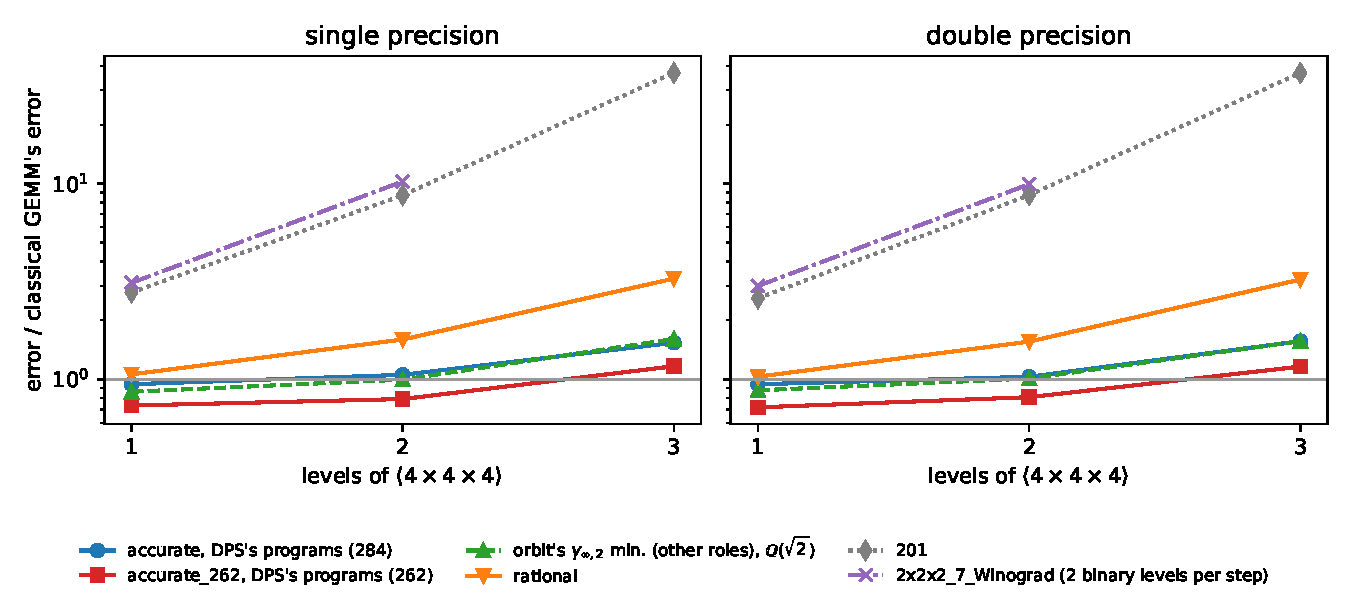
\includegraphics[width=\textwidth]{acc262_levels.pdf}
\caption{Mean error against the exact reference as a multiple of the
classical GEMM's error, over all sizes, distributions and seeds of the
main campaign ($n=4096$ and $8192$).  The points for
\texttt{2x2x2\_\allowbreak 7\_\allowbreak Winograd} are two and four binary levels.}
\label{fig:levels}
\end{figure}

\subsection{Deep recursion}\label{sec:deep}

To see the growth factors at work we recursed down to scalars: $n=1024$
with one to five levels (leaves $256$, $64$, $16$, $4$ and $1$), as in
DPS's experiments~\cite[Fig.~1]{DPS26a}, ten instances per precision.
Table~\ref{tab:deep} gives the results and Figure~\ref{fig:deep} plots
them.
\begin{itemize}
\item \acct with DPS's programs is again the most accurate from two
  levels on, and at one level in double precision; at one level in
  single precision probe~A and our programs for \acct have $0.78$
  against its $0.79$.  Its advantage over \acc grows with depth: its error is
  $0.80$--$0.83$ of \acc's at one level and $0.72$ at five (single
  instances $0.67$--$0.80$), in both precisions.
\item From four levels to five, the errors grow by $2.60$--$2.61$ for
  \acct and $2.75$--$2.79$ for \acc, about $6\%$ slower per level.  That is the direction $\ginf$ predicts, but less than its ratio
  $16\sqrt2/18\sqrt2=8/9$ would give.
\item Programs matter more at depth.  \acct with our $445$-operation
  programs and the two probes beat \acc in the main campaign, where the
  leaves are larger, but at $n=1024$ they fall behind \acc with DPS's
  programs from three levels on: $2.12$--$2.29$ against $2.00$ at three
  levels and $13.96$--$15.45$ against $13.29$ at five, in single
  precision.  Only \acct with DPS's programs beats \acc at every depth.
  Section~\ref{sec:disc} explains why.
\item Among the direct-sum programs, the dyadic probes stay $24$--$29\%$
  below \acc's at five levels and the orbit's $\ginf$ minimum only about
  $8\%$: the rounding of its constants compounds with depth.
\item \rat grows by about $3.6$ per level, \pto by
  about $7.5$, and \texttt{2x2x2\_\allowbreak 7\_\allowbreak Winograd} by about $7$ per two binary levels.
\end{itemize}

% generated by matmul/fastmm/paper_acc262.py --deep from accuracy_deep_2026-10-25.txt
\begin{table}[t]
\centering
\caption{Deep recursion at $n=1024$: mean error against the exact reference as a multiple of the classical GEMM's error, over ten instances per precision (uniform and normal, five seeds each); five levels reach scalar leaves.  Winograd: twice as many binary levels.}
\label{tab:deep}
\footnotesize
\setlength{\tabcolsep}{3.5pt}
\begin{tabular}{lrrrrrrrrrr}
\toprule
 & \multicolumn{5}{c}{single precision} & \multicolumn{5}{c}{double precision}\\
\cmidrule(lr){2-6}\cmidrule(lr){7-11}
levels & 1 & 2 & 3 & 4 & 5 & 1 & 2 & 3 & 4 & 5\\
\midrule
\texttt{accurate} (284) & 0.95 & 1.10 & 2.00 & 4.77 & 13.29 & 0.91 & 1.18 & 2.09 & 4.91 & 13.50\\
\texttt{accurate\_262} (262) & 0.79 & 0.97 & 1.67 & 3.75 & 9.79 & 0.76 & 0.98 & 1.63 & 3.68 & 9.58\\
\texttt{accurate\_262} point (445) & 0.78 & 1.10 & 2.29 & 5.71 & 15.45 & 0.78 & 1.09 & 2.20 & 5.48 & 15.62\\
\texttt{accurate}, direct & 1.00 & 1.35 & 2.69 & 6.76 & 19.63 & 0.95 & 1.29 & 2.57 & 6.62 & 19.36\\
probe A & 0.78 & 1.08 & 2.27 & 5.40 & 14.91 & 0.80 & 1.09 & 2.21 & 5.43 & 14.45\\
probe B & 0.82 & 1.08 & 2.12 & 5.28 & 13.96 & 0.82 & 1.05 & 2.12 & 5.10 & 14.05\\
$\gamma_{\infty,2}$ min., $\mathbb{Q}(\sqrt2)$ & 0.89 & 1.22 & 2.40 & 6.42 & 18.06 & 0.92 & 1.20 & 2.36 & 5.89 & 17.57\\
\texttt{rational} & 1.08 & 1.92 & 4.76 & 15.48 & 56.64 & 1.13 & 1.90 & 4.80 & 15.36 & 55.20\\
\texttt{201} & 2.75 & 9.86 & 48.87 & 304 & 2242 & 2.89 & 9.60 & 47.50 & 301 & 2293\\
\midrule
\texttt{Winograd} & 2.88 & 10.46 & 46.34 & 254 & 1726 & 3.38 & 11.14 & 47.75 & 248 & 1753\\
\bottomrule
\end{tabular}
\end{table}

% accurate_262/accurate by level (single; double): 1: 0.799 [0.670,0.889] 0.829; 2: 0.845 [0.748,0.948] 0.835; 3: 0.828 [0.706,0.959] 0.789; 4: 0.764 [0.646,0.822] 0.756; 5: 0.724 [0.670,0.803] 0.715
% growth 3->4 4->5 (single; double) bench_fmm: 2.39 2.79; 2.35 2.75
% growth 3->4 4->5 (single; double) bench_fmm_acc262: 2.24 2.61; 2.26 2.60
% growth 3->4 4->5 (single; double) bench_fmm_var_g16s2o: 2.50 2.70; 2.49 2.85
% growth 3->4 4->5 (single; double) bench_fmm_var_table1d: 2.51 2.90; 2.57 2.92
% growth 3->4 4->5 (single; double) bench_fmm_var_probeA: 2.38 2.76; 2.46 2.66
% growth 3->4 4->5 (single; double) bench_fmm_var_probeB: 2.50 2.64; 2.41 2.76
% growth 3->4 4->5 (single; double) bench_fmm_var_g214d: 2.67 2.81; 2.50 2.98
% growth 3->4 4->5 (single; double) bench_fmm_orig: 3.25 3.66; 3.20 3.59
% growth 3->4 4->5 (single; double) bench_fmm_201: 6.22 7.38; 6.33 7.62


\begin{figure}[t]
\centering
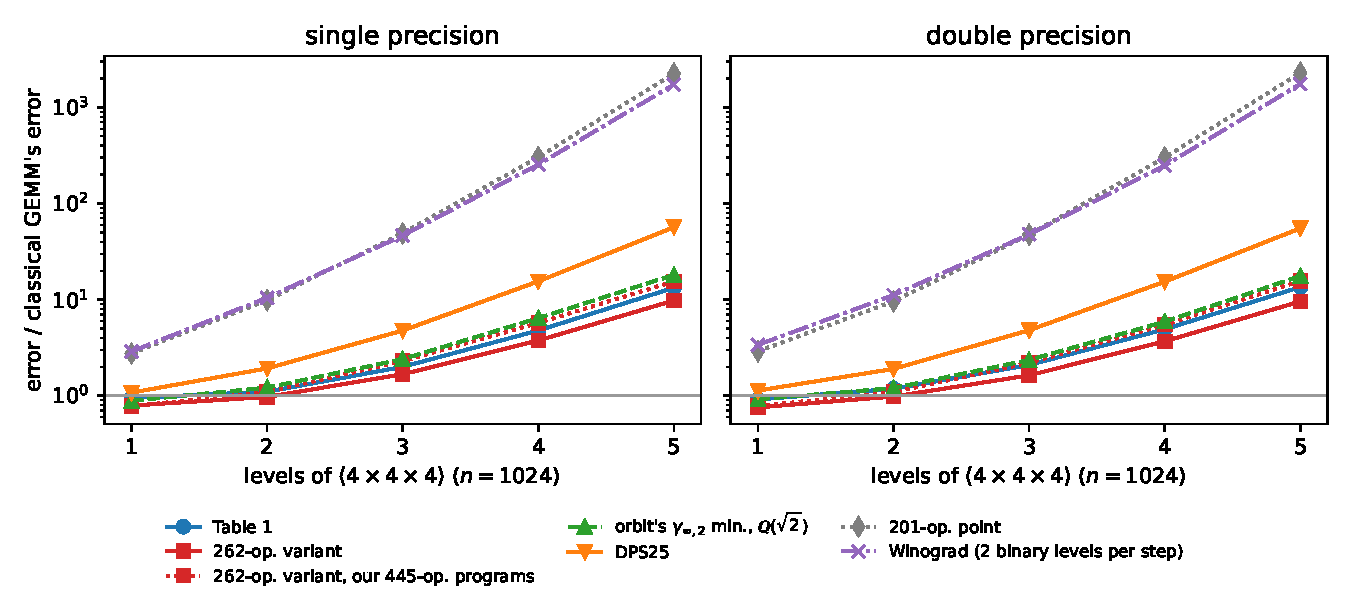
\includegraphics[width=\textwidth]{acc262_deep.pdf}
\caption{Deep recursion at $n=1024$: mean error against the exact reference as a multiple of the classical GEMM's error, over ten instances per precision.  The points for \texttt{2x2x2\_\allowbreak 7\_\allowbreak Winograd} are two binary levels per step.}
\label{fig:deep}
\end{figure}



\section{Speed}\label{sec:speed}

Table~\ref{tab:speed} times DPS's programs in our library.  It
covers single levels with one GEMM at a time (\texttt{D48/G}) and the
plans the library picks at these sizes, which use six GEMM streams and
pipelined passes (\texttt{D48/G6}, \texttt{D48+4/D48/G6}), in
alternating rounds.  Both take the same time to within the timer's
resolution ($0.977$--$1.007$).  The passes move the same data, and with
$262$ against $284$ operations neither is bound by arithmetic.  Our
$445$-operation programs for \acct also took \acc's time.  In an
earlier run of three alternating rounds of five, their fastest run was
$0.998$--$1.007$ times \acc's in seven of the eight configurations, and
$1.041$ in the eighth (double precision, \texttt{D48/G6}, $n=4096$),
where the medians of the rounds vary by up to $10\%$.  Their passes are
slower, $0.057$ against $0.054$--$0.055$~s at $n=8192$ in double
precision, but the passes take only $5$--$17\%$ of the time.  So the more accurate algorithm
costs nothing at run time, and it is the cheaper one in operation count.

\section{Discussion}\label{sec:disc}

% generated by matmul/fastmm/paper_acc262.py --model from accuracy_campaign_2026-10-25.txt and accuracy_deep_2026-10-25.txt
\begin{table}[tb]
\centering
\caption{The first-order rounding model of one level of each program (Section~\ref{sec:disc}) beside the measured errors.  L+R and P: the RMS error those passes add, mean over the outputs; worst: all passes, worst output; all three relative to an output's RMS, in units of one rounding.  Count and size: the roundings of the P pass that reach an output and their RMS size in output units (value times weight), means over the outputs; an output's P error is $\sqrt{\mathrm{count}}$ times the size.  Amp.: how much the worst output amplifies the leaf products' own errors, a property of the scheme.  The last two rows are the best program sets of the optimizer sweep (Section~\ref{sec:disc}), modelled but not measured.  Measured: single-precision error as a multiple of the classical GEMM's at three levels (Table~\ref{tab:acc}) and five (Table~\ref{tab:deep}).}
\label{tab:model}
\footnotesize
\setlength{\tabcolsep}{4pt}
\begin{tabular}{lrrrrrrrr}
\toprule
 & \multicolumn{6}{c}{model, one level} & \multicolumn{2}{c}{measured}\\
\cmidrule(lr){2-7}\cmidrule(lr){8-9}
program & L+R & P & count & size & worst & amp. & 3 levels & 5 levels\\
\midrule
\texttt{accurate\_262}, DPS's programs (262) & 5.74 & 3.09 & 15.0 & 0.80 & 7.22 & 2.83 & 1.17 & 9.79\\
\texttt{accurate\_262}, model-searched programs (539) & 5.52 & 2.97 & 15.0 & 0.77 & 6.47 & 2.83 & 1.18 & 9.25\\
\texttt{accurate\_262}, our programs (445) & 5.61 & 8.22 & 35.6 & 1.39 & 12.51 & 2.83 & 1.33 & 15.45\\
probe B, direct sums & 7.19 & 7.42 & 29.0 & 1.38 & 10.75 & 2.83 & 1.26 & 13.96\\
probe A, direct sums & 10.12 & 5.67 & 15.0 & 1.46 & 11.77 & 2.83 & 1.32 & 14.91\\
\texttt{accurate}, DPS's programs (284) & 5.57 & 3.35 & 18.0 & 0.79 & 7.12 & 3.16 & 1.54 & 13.29\\
\texttt{accurate}, direct sums & 7.64 & 5.98 & 18.0 & 1.41 & 11.14 & 3.16 & 1.65 & 19.63\\
\texttt{rational}, DPS's programs (315) & 7.75 & 7.11 & 47.8 & 1.04 & 11.73 & 4.00 & 3.27 & 56.64\\
\texttt{201}, our programs (201) & 12.30 & 8.87 & 22.7 & 1.85 & 21.05 & 9.53 & 36.84 & 2242\\
\midrule
\texttt{accurate\_262}, DPS's scheme, sweep (348) & 7.05 & 3.15 & 15.0 & 0.81 & 8.95 & 2.83 & -- & --\\
\texttt{accurate\_262}, our scheme, sweep (409) & 7.39 & 3.40 & 15.0 & 0.88 & 9.96 & 2.83 & -- & --\\
\bottomrule
\end{tabular}
\end{table}



\paragraph{What predicts the measured error.}
Table~\ref{tab:factors} sets the factors beside the error measured at
three levels in single precision, where the schemes differ most.  The
growth factors separate the distant schemes (\rat, \pto, two levels
of \texttt{2x2x2\_\allowbreak 7\_\allowbreak Winograd}), but no single factor orders the close ones.
\begin{itemize}
\item Probe~A has \acct's $\ginf$ but a larger measured error.
\item Probe~B has a larger $\ginf$ than \acc but a smaller measured
  error.
\item The orbit's $\ginf$ minimum, in another role, has the smallest
  $\ginf$ of all but
  about the same measured error as \acc.
\end{itemize}
Among the dyadic schemes, $Q_0$ does not order the measured errors
either: $34$, $46$, $40$ and $46$ for \acct, probe~B, probe~A and
\acc.  The term count $T_0$ of~(\ref{eq:t0}) does, $80$, $94$, $144$
and $180$, on these four points.  Of the dyadic schemes, \acct is best
or tied for best in every factor, and with DPS's programs its measured
error is the smallest.


\paragraph{Dyadic coefficients.}
The orbit's $\ginf$ minimum and probe~A have nearly the same $\ginf$
($21.41$ and $22.63$) and $Q_0$ ($42$ and $40$), and the former has
the smaller $\giinf$ ($176.6$ against $256$).  Yet the former's measured
error is about $20\%$ larger at three levels: $1.61$ against $1.32$ times the
classical error in single precision, and $1.57$ against $1.36$ in double.  Its constants, such as $2(\sqrt2-1)$,
are rounded to the working precision, so the scheme itself is inexact by
a unit roundoff, and each multiplication by them rounds.  Multiplications
by $\pm1/2^k$ are exact.  The gap compounds with depth: at five levels
the probes are $24$--$29\%$ below \acc's direct sums and the
$\Q(\sqrt2)$ point only $8\%$.  A search for accuracy should therefore
keep to small dyadic coefficients, and its programs to scalings by
powers of two.

\paragraph{Programs.}
The same scheme has different measured errors with different
programs.  \acct with DPS's programs beats \acct with ours, and \acc
with DPS's programs beats \acc as direct sums
($1.17$ against $1.33$, and $1.54$ against $1.65$, times the classical
error at three levels in single precision).  Our scheme for \acct is
equivalent to DPS's by relabelling and by scalings by powers of two,
which are exact in floating point, so the first difference lies entirely
in the programs.  It is not their length.  DPS's programs have the
longer chains of roundings, up to $22$ through one level against $18$
for ours, and the probes' direct sums have $37$ and $39$ yet beat our
programs (Table~\ref{tab:model}).  Nor is the second difference the
direct sums' multiplications by $3/4$: in the model below they change
the result by under $1\%$.

\paragraph{A rounding model.}
Table~\ref{tab:model} models one level of each program to first order.
Every addition, and every scaling by a constant that is not a power of
two, rounds, with an error proportional to the exact value rounded, and
the errors are independent.  The inputs are independent with unit
variance, so the products have covariance
$(L_i\cdot L_{i'})(R_i\cdot R_{i'})$ and the size of every intermediate
value, cancellation included, is an exact second moment.  Propagating
each rounding to the outputs gives the error each pass adds to a level.
\begin{itemize}
\item For \acct, DPS's programs and ours add about the same error in the
  $L$ and $R$ passes ($5.74$ against $5.61$) but not in the $P$ pass
  ($3.09$ against $8.22$).  The sixteen products that feed an output
  are each $1/\sqrt2$ of its size and would sum to $2\sqrt2$ times its
  size if they did not cancel.  DPS's $P$ pass keeps its partial sums
  small: each output collects $15$ roundings whose RMS size is $0.80$ of
  the output's.  Ours lets them grow: each output collects $36$
  roundings, since our program shares more partial sums between
  outputs, of RMS size $1.39$.
\item At one level the leaf products' own errors dominate, and the two
  programs measure the same.  Every further level amplifies those by the
  same factor and adds a new pass error, so the gap grows with depth
  (Table~\ref{tab:deep}).
\item For the four programs whose schemes amplify leaf errors equally
  ($2\sqrt2$ for the worst output), the model's worst-output error
  orders the measured errors exactly, at three levels and at five.
\item \acc, \rat and \pto amplify leaf errors more ($3.16$, $4$ and
  $9.53$).  \acc's own programs add no more error than \acct's ($7.12$
  against $7.22$); its larger measured error comes from its scheme's
  larger amplification.  The same trade-off explains the crossover of
  Section~\ref{sec:deep}: the probes and our programs for \acct amplify
  less than \acc but add more error per level ($10.75$--$12.51$ against
  $7.12$), so they beat \acc while the leaves' own errors dominate and
  fall behind it at depth.
\end{itemize}

\paragraph{What the optimizer reaches.}
To see whether more search would have given us DPS's programs, we swept
PLinOpt's \texttt{optimizer} over both schemes and all three matrices:
$1000$ and $5000$ random loops instead of $100$, its exhaustive
nullspace permutations (\texttt{-N}), its factoring method (\texttt{-A}),
and for $P$ both direct optimization and the transposition pipeline.
Its exhaustive CSE search (\texttt{-E}) did not finish within $120$~s on
any matrix.  The best complete sets have $348$ operations for DPS's
scheme and $409$ for ours, against DPS's $262$ and our $445$.  So the
$262$-operation programs did not come from this search alone, and the
commit does not say how they were made.  The sweep did show where our
$P$ pass went wrong: every $P$ program optimized directly, rather than
through the transposition pipeline, has DPS's structure, $15$ roundings
per output of RMS size $0.81$--$0.88$, and adds $3.15$--$3.40$ against
their $3.09$ in the model (Table~\ref{tab:model}, last two rows).  Our
$L$ and $R$ programs still add more than DPS's ($7.05$--$7.39$ against
$5.74$), so the best sets model at $8.95$ and $9.96$ on the worst
output, between our $12.51$ and DPS's $7.22$.  We have not measured
these programs.

\paragraph{Recommendation.}
Wherever \acc is used, \acct is
better on both counts: $22$ fewer operations and about a quarter less
error, in the same orbit and with the same $\gamma_2$.

\paragraph{Limitations.}
\begin{itemize}
\item The measurements come from one machine and one implementation
  style: fused passes over a vendor GEMM, with large leaves.  The inputs
  are i.i.d.\ uniform or normal matrices, the error is the max-norm error
  relative to $\max\lvert C\rvert$, and there are at most three levels
  at $n=4096$ and $8192$ and five at $n=1024$.  Structured or badly scaled inputs may rank the
  schemes differently.
\item The continuous search gives no proof of global optimality.  Only
  the dyadic orthogonal moves are enumerated exhaustively;
  non-orthogonal dyadic isotropies, such as shears and scalings by two,
  are not.
\end{itemize}

\paragraph{Outlook.}
The natural next objective combines the growth factors with $Q_0$ and
the operation count over dyadic points, or uses the measured error of
deep recursion directly; \texttt{gamma48} makes such searches cheap.
Section~\ref{sec:beyond} carries the rounding model into a program
search, finds the scheme's amplification of the leaf error at its
floor, and lowers the deep-recursion error by a third with
double-precision passes.  Lower precisions (bf16, fp16), where every
level's error is a larger share of the result, are where an accurate
scheme matters most.

\section{Beyond the published programs}\label{sec:beyond}

The model of Section~\ref{sec:disc} points to two ways to a realized
algorithm more accurate than \acct with DPS's programs: programs that add
less rounding error, and schemes that amplify the leaf products' error
less.  We tried both; then the one lever that remained.

\subsection{Programs found with the model}\label{sec:searchprog}

\texttt{slpopt} (Rust) ports the model, exact to every printed digit of
Table~\ref{tab:model}, and searches programs of one matrix with the other
two fixed: programs are DAGs of sums and scalings, the moves keep every
output's linear form (rebuilding a sum tree at random or by smallest
partial sums, rotating, sharing and unsharing a sum, creating a common
subexpression across trees), simulated annealing drives them, and every
accepted move is checked against the matrix.  PLinOpt's
\texttt{optimizer}, which we made $7$--$10$ times faster for this
purpose (Section~\ref{sec:data}), supplies starting programs by the
thousand.

The headroom is small.  Of $3000$ random \texttt{optimizer} programs
per matrix, scored with the other two matrices at DPS's programs, the
best $R$ models at $6.56$ against DPS's $7.22$, $L$ gives one program
($7.27$, no ties to break) and no $P$ beats DPS's; the optimizer's
kernel and LU methods, annealing from DPS's programs, and a greedy
construction that applies the model-best subexpression at each step do
no better.  The best set we assembled, DPS's $L$, the best sampled $R$
after annealing, and a $P$ built by pairing the smallest partial sums
first, models at $6.47$ ($L$+$R$ $5.52$, $P$ $2.97$; $539$ operations;
SLPchecker passes all three).  Measured with the protocol of
Section~\ref{sec:acc} (the rows ``model-searched programs'' of
Tables~\ref{tab:acc}, \ref{tab:deep} and~\ref{tab:model}), its error is
$1.001$, $1.007$ and $1.014$ of \acct's at one to three levels, within
the seed-to-seed spread, and $0.95$ at four and five levels, at the same
speed.  Eleven percent less pass error is five percent at depth and
nothing with large leaves: the error that dominates is the leaf
products' own, amplified by the scheme.

\subsection{The amplification of the leaf error is at its minimum}\label{sec:ampfloor}

In the model, one level amplifies the leaf products' errors into output
$j$ by
\begin{equation}\label{eq:amp}
\mathrm{amp}_j=\tfrac12\Bigl(\sum_i p_{j,i}^2\,\lVert L_i\rVert_2^2\,
\lVert R_i\rVert_2^2\Bigr)^{1/2},
\end{equation}
the column ``amp.''\ of Table~\ref{tab:model}; \acct has $2\sqrt2$ for
every output, \acc $3.16$.  It is the root-sum-square counterpart of
$\ginf$'s per-output sum
$\sum_i\lvert p_{j,i}\rvert\,\lVert L_i\rVert_2\lVert R_i\rVert_2$: the
growth factor bounds the error with every rounding aligned, the model
adds independent roundings in quadrature.  For \acct each output
collects sixteen products with $\lvert p_{j,i}\rvert=1$ and
$\lVert L_i\rVert_2\lVert R_i\rVert_2=\sqrt2$, so the sum is $16\sqrt2$
and the root-sum-square $\frac12\sqrt{16\cdot2}=2\sqrt2$.  We looked
for less in every way we could:
\begin{itemize}
\item Over the $648$ dyadic orthogonal points of Section~\ref{sec:dyadic},
  each scored with greedy programs, $\mathrm{amp}$ takes five values:
  $2\sqrt2$ at $342$ points, \acct's among them, then $3.16$, $3.32$,
  $3.46$ and $3.74$.  The realized pass error ranges from $6.7$ to $8.6$,
  \acct's point at $6.96$ and the lowest, $6.73$, in probe~B's family.
\item Simulated annealing over non-orthogonal dyadic isotropies (shears
  by $\pm1$, $\pm\frac12$, $\pm2$, row swaps, scalings by $2^{\pm1}$)
  never leaves $2\sqrt2$, and BFGS over all $48$ parameters of the orbit
  from twelve random starts returns to $2\sqrt2$ at orthogonal points
  with all sixteen outputs equal.  The orbit's $\ginf$ minimum, $21.41$,
  has $\mathrm{amp}=3.14$: it minimizes the sum ($21.41$ against
  $22.63$) but not the root-sum-square ($3.14$ against $2.83$); a
  smaller growth factor is not a smaller amplification.
\item Over the whole variety of rank-$48$ decompositions of the
  $4\times4\times4$ tensor, minimizing a soft maximum of the
  $\mathrm{amp}_j$ with the Brent equations as a penalty raised in
  stages (L-BFGS on all $2304$ coefficients), every start returns to
  $2\sqrt2$: sixteen starts from \acct perturbed by up to the size of
  its coefficients land on generic points of its orthogonal sub-orbit
  ($\gamma_2=154.51$, dense irrational coefficients), and starts from Li,
  Wang and Hu's $s(1/2)$, whose own orbit bottoms at $3.00$, leave that
  orbit for $2\sqrt2$ too.
\item The other known classes, minimized over their orbits: $s(1/4)$,
  the DPS class, $2.83$; $s(1/2)$ $3.00$; $s(1)$ $3.54$; $s(2)$ $4.50$;
  $s(4)$ $6.01$; $s(8)$ $8.25$; Agarwal's scheme $5.80$.
\end{itemize}
The minimum set is the orthogonal sub-orbit on which $\gamma_2$ is
minimal, which is where DPS looked first.  This is not a proof that
$2\sqrt2$ is the floor for rank $48$, but it is every basin we have a
foothold in, and it closes the scheme as a lever for this measurement:
whatever the program, one level of a known rank-$48$ scheme multiplies
the leaf error by at least $2\sqrt2$.

\subsection{Double-precision passes}\label{sec:f64pass}

The remaining lever is the passes' arithmetic.  With \texttt{FMM\_F64PASS=1}
the library's $4\times4$ passes on the single-precision path read and
write \texttt{float} blocks but add in \texttt{double} (a third kernel
set, generated like the others), so a pass rounds once per element it
stores, at the GEMM's interface, instead of at every addition; the GEMMs
and the plans are unchanged.  The interface roundings are amplified
like the leaf error, so the pass term cannot vanish: one rounding per
stored element gives, in the model, $L$+$R$ $4.0$ and $P$ $1.0$, a worst
output of $4.1$ against DPS's programs' $7.2$.

Measured with DPS's programs both ways (the rows ``f64 passes'' of
Tables~\ref{tab:acc} and~\ref{tab:deep}, and the dashed line of
Figure~\ref{fig:deep}), the error with the double-precision passes is
$0.99$, $1.02$ and $0.98$ of the single-precision passes' at one to
three levels on $n=4096$ and $8192$, a tie where the leaves' error
dominates, and $0.97$, $0.96$, $0.85$, $0.72$ and $0.64$ at one to five
levels on $n=1024$: $6.25$ times the classical error at five levels
instead of $9.79$.  The passes are memory-bound, so the double
arithmetic is nearly free: $1.000$--$1.017$ of the time on the plans at
$4096$ and $8192$ and on one level at $16384$, and $1.057$ on the
three-level pipelined plan at $16384$, where the passes are the largest
share.  This is the first change that lowers the deep-recursion line,
and the model's floor accounts for its size.  The library leaves the
switch off by default; the natural rule is to turn it on with the
accuracy budget, for plans of three or more fast levels.

\section{Data and code}\label{sec:data}

Everything is in the public repository
\url{https://github.com/gsidebottom/logic}; paths below are relative to
it.
\begin{itemize}
\item The search: \path{src/bin/gamma48.rs} (the continuous search) and
  \path{matmul/dps48/gamma/}, which holds the role assignments and the
  isotropy action (\path{orbit.py}), the earlier Python search
  (\path{search_orth.py}, \path{search_gl.py}), the exact constructions
  (\path{exact.py}), the exhaustive dyadic enumeration
  (\path{dyadic_orth.py}) and the equivalence test (\path{equiv.py},
  \path{equiv262.py}).
\item Growth factors: \path{matmul/fastmm/growth.py}, checked against
  PLinOpt's \texttt{growthfactor}.
\item Other classes: \path{matmul/dps48/lwh_family.py} and
  \path{agarwal_replacement.py}, which rebuild the Li--Wang--Hu members and
  Agarwal's scheme from the papers.
\item Measurements: \path{matmul/fastmm} (\path{bench_fmm.c},
  \path{bench_impl.h}, \path{gen_kernels.py}).  The builds are
  \path{build/bench_fmm_acc262} for the $262$-operation programs and
  \path{build/bench_fmm_acc284} for \acc's.  The runs labelled
  \texttt{bench\_fmm} in the result files used \acc's programs, the
  library's default until it switched to \acct
  after these measurements.  \texttt{FMM\_EXACT}, \texttt{FMM\_NORMAL}
  and \texttt{FMM\_SEED} select the reference, the distribution and the
  instance, and \texttt{FMM\_REFCACHE} shares references between
  builds.  The probes' programs are in \path{matmul/dps48/gamma/slp/}.
  Raw results are in \path{matmul/fastmm/results/}
  (\path{accuracy_campaign_2026-10-25.txt},
  \path{accuracy_deep_2026-10-25.txt}, \path{gamma_search_2026-10-25.txt},
  \path{gamma_classes_2026-10-25.txt}), and
  \path{matmul/fastmm/paper_acc262.py} turns them into this paper's
  tables and figures.
\item The rounding model: \path{matmul/dps48/gamma/slp_errmodel.py}, with
  its output in \path{matmul/fastmm/results/slp_errmodel_2026-10-25.txt};
  \path{paper_acc262.py --model} writes Table~\ref{tab:model}.
\item Section~\ref{sec:beyond}: \path{src/bin/slpopt.rs} (the model,
  the program search, \texttt{realized} scoring); the program sets
  \path{matmul/dps48/gamma/slp/opt1_{L,R,P}.slp}; the amplification
  floor by \path{matmul/dps48/gamma/dyadic_points.py}, \path{ampwalk.py},
  \path{ampmin.py}, \path{ampvariety.py} and \path{inspect_point.py},
  with the other classes' schemes in \path{matmul/dps48/classes/} and
  results in \path{matmul/fastmm/results/} (\path{dyadic_points_realized_},
  \path{amp_floor_}, \path{amp_classes_} and \path{amp_variety_2026-10-26.txt});
  the double-precision passes in
  \path{matmul/fastmm/gen_kernels.py}, \path{fmm.c} and \path{fmm_impl.h}
  (\texttt{FMM\_F64PASS}); the campaigns \path{campaign_var.sh},
  \path{campaign_f64pass.sh} and \path{summarize_var.py}, with their logs
  \path{accuracy_opt1_}, \path{accuracy_deep_opt1_}, \path{accuracy_f64pass_},
  \path{accuracy_deep_f64pass_} and \path{speed_*_2026-10-26.txt}.  The
  faster PLinOpt optimizer (one generator per thread with a seed option,
  no transposed copy per subexpression, incremental pair bookkeeping, a
  word-size prime field with rational reconstruction, $7$--$10$ times
  faster on these matrices) is the branch \texttt{optimizer-speed} of
  \url{https://github.com/gsidebottom/plinopt}.
\item The optimizer sweep: \path{matmul/dps48/gamma/optsweep.sh} and
  \path{optsweep_score.py}; its log and scores are in
  \path{matmul/fastmm/results/optimizer_sweep_2026-10-26.txt} and its
  best programs in \path{matmul/dps48/gamma/slp/sweep_{dps,ours}_{L,R,P}.slp}.
\item The schemes: PLinOpt's \texttt{data/4x4x4\_48\_accurate\_262} and
  \texttt{data/4x4x4\_48\_accurate}~\cite{PLinOpt}; our scheme equivalent to \acct
  is \path{matmul/dps48/gamma/g16s2_{L,R,P}.sms} and our programs for it
  \path{matmul/dps48/gamma/slp/g16s2o_{L,R,P}.slp}.
\item The orbit's $\ginf$ minimum (Section~\ref{sec:search}): the
  direct-sum programs we measured, with rounded constants,
  \path{matmul/dps48/gamma/slp/g214d_{L,R,P}.slp}; the search's $(U,V,W)$
  that reach it from \acc in roles~1 and~2, the first lines of
  \path{matmul/dps48/gamma/rs_table1_r1.txt} and \path{rs_table1_r2.txt}
  (the value, the start's seed, then $U$, $V$, $W$ row by row); and its
  exact form in $\Q(\sqrt2)$, \path{matmul/dps48/gamma/g214_exact_{L,R,P}.txt}
  (one entry $a+b\sqrt2$ per line as \texttt{row col a b}) with the
  readable listing \path{g214_exact.txt}, both written and checked by
  \path{exact_q214.py}.
\end{itemize}

\section*{Acknowledgments}

This work was carried out in an interactive collaboration with Claude
(Anthropic; the Opus~5.5 and Fable~5.1 models), which implemented the search,
measurement and verification tools and much of this text under the
author's direction and review.  Every claim is checked mechanically by
the tools listed above; the results rest on those checks rather than on
trust in either the author or the tools.  The algorithm comes from
Dumas, Pernet and Sedoglavic's work and was published by J.-G.~Dumas in
PLinOpt; our search found a scheme equivalent to it, and we learned
that it was already there only after constructing ours.  We thank
Alexandre Sedoglavic for his comments on the first draft: the
parametrization of the orbit search in Section~\ref{sec:search}, Touko
Ursin's priority on the $16\sqrt2$ point, and the place of the orbit's
$\ginf$ minimum in the abstract all come from them~\cite{Sedoglavic26};
the account of how \acct was constructed and the numbering of the
equations come from his second message~\cite{Sedoglavic26b}.

{\small
\begin{thebibliography}{99}
\bibitem{Agarwal26} A.~Agarwal, \emph{Certified local rank and
uniqueness barriers for a 48-term matrix-multiplication decomposition},
arXiv:2609.13596 (2026).
\bibitem{BBDLS16} G.~Ballard, A.~R.~Benson, A.~Druinsky, B.~Lipshitz,
O.~Schwartz, \emph{Improving the numerical stability of fast matrix
multiplication}, SIAM J.\ Matrix Anal.\ Appl.\ 37 (2016) 1382--1418.
\bibitem{BL80} D.~Bini, G.~Lotti, \emph{Stability of fast algorithms for
matrix multiplication}, Numer.\ Math.\ 36 (1980) 63--72.
\bibitem{Brent70} R.~P.~Brent, \emph{Algorithms for matrix
multiplication}, Technical Report STAN-CS-70-157, Stanford University
(1970).
\bibitem{vanElfrinkhof1897} L.~van Elfrinkhof, \emph{Eene eigenschap
van de orthogonale substitutie van de vierde orde}, Handelingen van het
6e Nederlandsch Natuurkundig en Geneeskundig Congres, Delft (1897).
\bibitem{deGroote78} H.~F.~de~Groote, \emph{On varieties of optimal
algorithms for the computation of bilinear mappings I. The isotropy
group of a bilinear mapping}, Theoret.\ Comput.\ Sci.\ 7 (1978) 1--24.
\bibitem{DDHK07} J.~Demmel, I.~Dumitriu, O.~Holtz, R.~Kleinberg,
\emph{Fast matrix multiplication is stable}, Numer.\ Math.\ 106 (2007)
199--224.
\bibitem{DPS24} J.-G.~Dumas, C.~Pernet, A.~Sedoglavic, \emph{Strassen's
algorithm is not optimally accurate}, Proc.\ ISSAC 2024, 254--263.
\bibitem{DPS25} J.-G.~Dumas, C.~Pernet, A.~Sedoglavic, \emph{A
non-commutative algorithm for multiplying $4\times4$ matrices using
$48$ non-complex multiplications}, arXiv:2506.13242 (2025).
\bibitem{DPS26a} J.-G.~Dumas, C.~Pernet, A.~Sedoglavic, \emph{A more
accurate rational non-commutative algorithm for multiplying $4\times4$
matrices using $48$ multiplications}, arXiv:2603.18699 (v1 19~March
2026, v3 29~July 2026).
\bibitem{DPS26b} J.-G.~Dumas, C.~Pernet, A.~Sedoglavic, \emph{Towards
automated generation of fast and accurate algorithms for recursive
matrix multiplication}, J.\ Symbolic Comput.\ 134 (2026) 102524.
\bibitem{DPSST26} J.-G.~Dumas, C.~Pernet, A.~Sedoglavic, J.~Stapleton,
P.~Tichavsk\'y, \emph{Fast matrix multiplication via recursive
$\langle4\times4\times4:48\rangle$ algorithms into practice},
arXiv:2609.12027 (v1 10~September 2026, v2 2~October 2026).
\bibitem{PLinOpt} J.-G.~Dumas, B.~Grenet, C.~Pernet, A.~Sedoglavic,
\emph{PLinOpt, a collection of C++ routines handling linear \&
bilinear programs}, \url{https://github.com/jgdumas/plinopt}; data
files \texttt{4x4x4\_48\_accurate} (commit \texttt{fb753b5}, 23~June
2026) and \texttt{4x4x4\_48\_accurate\_262} (commit \texttt{b441528},
13~October 2026).
\bibitem{Higham02} N.~J.~Higham, \emph{Accuracy and Stability of
Numerical Algorithms}, 2nd ed., SIAM, 2002.
\bibitem{LWH26} X.~Li, Y.~Wang, S.~Hu, \emph{Substitution and quotient
of the isotropy group action}, arXiv:2607.15069 (2026).
\bibitem{Novikov25} A.~Novikov et al., \emph{AlphaEvolve: a coding agent
for scientific and algorithmic discovery}, arXiv:2506.13131 (2025).
\bibitem{ORO05} T.~Ogita, S.~M.~Rump, S.~Oishi, \emph{Accurate sum and
dot product}, SIAM J.\ Sci.\ Comput.\ 26 (2005) 1955--1988.
\bibitem{Sedoglavic26} A.~Sedoglavic, private communication (e-mail
to the author), 26~October 2026: comments on the first draft of this
paper; the orbit search should be restricted to the factorization of
$GL_4$ by the orthogonal matrices for the growth factor, where a
convexity result ensures uniqueness, and to $SO(4)$ in Van Elfrinkhof's
parametrization for the other norms; the $\ginf=16\sqrt2$ point was
found by Touko Ursin in mid-September 2026 with Hadamard matrices.
\bibitem{Sedoglavic26b} A.~Sedoglavic, private communication (e-mail
to the author), 27~October 2026: how \acct was constructed (the
orbit's $\gamma_2$ minimum by numerical optimization over the quotient
of $GL_4$ by the orthogonal group, then Ursin's exploration of Hadamard
matrices for $\ginf$), and that the equations of this paper should be
numbered.
\bibitem{S26} G.~Sidebottom, \emph{201 operations for rank-48 $4\times4$
matrix multiplication over rings containing $1/2$}, preprint (2026);
PLinOpt data file \texttt{4x4x4\_48\_201}.
\bibitem{logic} G.~Sidebottom, \emph{logic}, source repository,
\url{https://github.com/gsidebottom/logic} (2026).
\end{thebibliography}
}

\end{document}
